Označimo, za početak, izvršno stanje programa u jednom momentu, pod čime se podrazumeva vrednost promenljivih kao i mesto u kodu do koga se došlo, odnosno na koje pokazuje programski brojač, sa $v \in V$ gde je $V$ skup svih takvih stanja. Tada možemo primetiti binarnu relaciju prelaska stanja $v_{0} \rightsquigarrow v_{1}$ koja predstavlja da stanje $v_{1}$ može uslediti za stanjem $v_{0}$. \footnote{Ovo poglavlje se primarno oslanja na \cite{salcianu}, gde se mogu naći dokazi tvrdnji koji su ovde izostavljeni radi sažetosti.} \\

Bitno je napomenuti da se ova relacija ne može zameniti funkcijom koja bi slikala jedno stanje u iduće, jer prelazak može zavisiti od okolnosti koje nisu definisane unutar programa, poput učitavanja podataka ili redosleda izvršavanja instrukcija u slučajevima kada program ima više niti, tako da može postojati više različitih stanja u koje jedno stanje prelazi. Posebno su nam zanimljiva stanja $$... \rightsquigarrow v_{n} \rightsquigarrow v_{n}$$ koja odgovaraju zaustavljanjima programa. \\
 
Budući da je u opštem slučaju jedini način da odredimo $v$ da izvršimo sam program, uopštićemo problem uvođenjem pojma prostora svojstava $L$. Njegovi elementi $l \in L$, koje nazivamo apstraktnim stanjima, obuhvataće svojstva koja stanja u koja program dospeva u datom trenutku imaju. Potrebno je naglasiti da dato apstraktno stanje ne predstavlja svojstva jednog konkretnog stanja, već više konkretnih stanja te da pojedinačne promenljive apstraktnih stanja uzimaju vrednosti iz partitivnog domena odnosno skupa podskupova domena promenljivih u konkretnim stanjima.\cite{denotationalsemantics} \\

Nad prostorom svojstava već možemo definisati funkciju $f_{L}:L\rightarrow L$ koja slika apstraktno stanje u ono koje mu sledi.

Pokazaće se korisno definisati dodatnu strukturu nad $L$: \\
\begin{definicija}
Neka je nad $L$ definisana relacija poretka, odnosno relacija $\sqsubseteq$ takva da za sve $a, b, c \in L$ važi
\begin{enumerate}
\item $a \sqsubseteq a$ (Refleksivnost)
\item ako su $a \sqsubseteq b$ i $b \sqsubseteq a$ tada $a = b$ (Antisimetričnost)
\item ako su $a \sqsubseteq b$ i $b \sqsubseteq c$ tada $a \sqsubseteq c$ (Tranzitivnost)
\end{enumerate}
Ukoliko za svaki podskup $L\prime \subseteq L$ postoji najmanja gornja granica $\bigsqcup L^{\prime}$ i najveća donja granica $\bigsqcap L^{\prime}$ tada se $L$ naziva \emph{potpunom mrežom}. \cite{algebra}
\end{definicija} 

\begin{figure}
\begin{center}
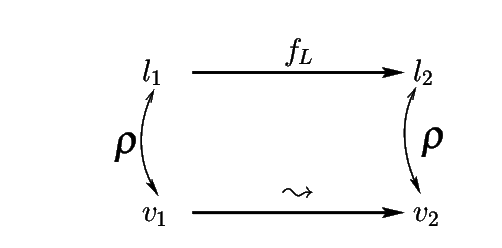
\includegraphics[scale=0.5]{Rho.png}
\end{center}
\caption{Odnos između apstraktnih i konkretnih stanja}
\label{fig:Rho}
\end{figure}

Relacija poretka koju uvodimo nad prostorom svojstava je takva da su veći elementi opštiji od manjih, odnosno da predstavljaju slabije tvrđenje o stanju programa. Tada $\bigsqcup L^{\prime}$ predstavlja disjunkciju apstraktnih stanja u $L^{\prime}$ odnosno stanje u kome važe bilo koja od datih svojstava, dok $\bigsqcap L^{\prime}$ označava stanje u kome sva svojstva važe. Bitne vrednosti su takođe i $\bigsqcup L = \top$ i $\bigsqcap L = \bot$.

Sada želimo dovesti u vezu konkretna stanja programa sa apstraktnim stanjima koja ih modeliraju putem relacije $\rho \subseteq V \times L$ kao što je prikazano na slici \ref{fig:Rho} \footnote{slika je preuzeta sa izmenama iz \cite{salcianu}}. Zahtevamo sledeće od ove relacije:
\begin{enumerate}
\item $\forall v,\, l_{1},\, l_{2},\, (v\: \rho \: l_{1}) \vee (l_{1} \sqsubseteq l_{2}) \Rightarrow (v\: \rho \: l_{2})$
\item $\forall v,\, L^{\prime} \subseteq L, (\forall l \in L^{\prime}, 	(v\: \rho \: l)) \Rightarrow v\: \rho \: (\bigsqcap L^{\prime})$
\end{enumerate}

Ovakvu relaciju nazivamo \emph{relacijom ispravnosti}. Da bi dokazali njenu valjanost u konkretnom slučaju, dovoljno je dokazati je za početno stanje izvršavanja i pokazat da se valjanost očuvava pri svakom prelasku u iduće stanje. 


\subsection{Fiksne tačke}
Ukoliko bismo želeli saznati svojstva programa $l$ u nekoj tački izvršavanja, najdirektniji i najprecizniji način bi bio da izračunamo sva apstraktna stanja $l_{i} \in W(l)$ dobijena duž putanja izvršavanja koja vode do te tačke od početnog stanja $l_{0}$ i zatim nađemo $\bigsqcup W(l) = l$. 

Nažalost, u praksi je takav račun nemoguć ili makar veoma zahtevan. Umesto toga, računaju se fiksne tačke funkcije $x = f_{L}(x)$ koje takođe čine potpunu mrežu pod uslovom da je $f_{L}$ \emph{monotona} \cite{tarski}, odnosno da važi $$\forall l_{1},\, l_{2},\, l_{1} \sqsubseteq l_{2} \, \Rightarrow \, f_{L}(l_1) \sqsubseteq f_{L}(l_2)$$ 

 Ako je uz to funkcija i \emph{neprekidna}, $\bigsqcup f_{L}[L^{\prime}] = f_{L}[\bigsqcup L^{\prime}]$, tada se najmanja fiksna tačka može izračunati kao $$\bigsqcup \{ \: f^{n}_{L}(\bot)\: \}_{n \in \mathbb{N}} \quad \text{gde je} \quad f^{0}_{L}(\bot) = \bot \quad \text{i} \quad f^{n}_{L}(\bot) = f_{L}(f^{n-1}_{L}(\bot)) \quad \cite{baranga}$$

Ipak, i ovom slučaju niz $f^{n}_{L} ( \bot )$ može previše sporo konvergirati, zbog čega uvodimo još jedan, grublji, prostor svojstava $M$ koji će služiti kao apstrakcija za $L$. Da bi objasnili odnos između ova dva prostora, moramo uvesti koncept galoaove veze:
\begin{definicija}
Neka su $(A, \geqslant)$ i $(B, \geqslant)$ parcijalno uređeni skupovi a $F : A \rightarrow B$ i $G : B \rightarrow A$ monotone funkcije. Tada je $\langle A, 	F, G, B \rangle$ \emph{galoaova veza} ukoliko važi 
\begin{enumerate}
\item $\forall a \in A, \, a \leqslant G (F (a))$ 
\item $\forall b \in B, \, b \geqslant F (G (b))$
\end{enumerate}
\end{definicija} 

\begin{teorema}
Ako između $L$ i $M$ postoji galoaova veza $\langle L, \alpha, \gamma, B \rangle$ tada je $\rho^{\prime} \subseteq M \times V$, takva da $$m\: \rho^{\prime}\: v \iff \gamma (m)\: \rho \: v$$ takođe relacija ispravnosti.
\end{teorema}

Druga tehnika je korišćenje operatora proširenja $\nabla : L \times L \rightarrow L$ takvog da je $x, y \sqsubseteq x \nabla y$ za sve $x, y$ i pomoću koga se za bilo koji rastući niz $(y_{n})_{n}$ može napraviti niz $$(x^{\prime}_{n})_{n} \quad \text{gde je} \quad x^{\prime}_{0} = y_{0} \quad \text{i} \quad x^{\prime}_{n} = x^{\prime}_{n-1} \nabla y_{n} $$ takav da konvergira u konačnoj broju koraka. \\

Najčešće za funkciju prelaska $f_{L}$ pravimo niz $(f^{n}_{\nabla})_{n}$ takav da:
$$
f^{n}_{\nabla} = 
\begin{cases}
\bot,            								  & 	\text{za} \quad n = 0 \\
f^{n-1}_{\nabla} 							      & \text{za} \quad n > 0 \quad \text{i} \quad f_{L}(f^{n-1}_{\nabla}) \sqsubseteq f^{n-1}_{\nabla} \\
f^{n-1}_{\nabla} \nabla f_{L}(f^{n-1}_{\nabla})  & \text{inače}
\end{cases}
$$

Ovime efektivno ubrzavamo nizove koji rastu a zaustavljamo ih u suprotnom, time se sprečava zaglavljivanje prilikom analizi petlji i drugih cikličnih tokova upravljanja. Za limes ovog niza ispostavlja se da je veći od najmanje fiksne tačke, te da ga dobro aproksimira. 
